% Set a pdf version and a document type
\ifx\pdfminorversion\undefined\else\pdfminorversion=4\fi
\documentclass[aspectratio=169,t,table]{beamer}

% Import all necessary packages
% Use this file to import all packages which are needed for the lecture
\usepackage[english]{babel}
\usepackage[utf8]{inputenc}
\usepackage[sfdefault]{roboto}
\usepackage[T1]{fontenc}
\usepackage{amsmath,amssymb}
\usepackage{graphicx}
\usepackage{listings}
\usepackage[backend=biber,sorting=none,doi=true,style=ieee]{biblatex}
\usepackage{url}
\usepackage{hyperref}
\usepackage{fontawesome5}
\usepackage{graphicx}
\usepackage{booktabs}
\usepackage{calc}
\usepackage{ifthen}
\usepackage{tabularx}
\usepackage{longtable}
\usepackage{makecell}
\usepackage{multicol}
\usepackage{multirow}
\usepackage{hhline}
\usepackage{qrcode}
\usepackage{xcolor}
\usepackage{cleveref}
\usepackage{tikz}
\usepackage{tikz-cd}
\usepackage{pgfplots,pgfplotstable,pgf-pie}
\usepackage[linesnumbered]{algorithm2e}
\usepackage{array}
\usepackage{mathtools}
\usepackage{verbatim}
\usetikzlibrary{patterns}
\usetikzlibrary{arrows.meta}


% Set the theme (customized FAU beamer theme)
\usetheme[%
	image,%
	longtitle,%
	inst=tf%
]{fau}

% Set all important settings and define commands that are used in more than one lecture
% Set institute and date 
\institute[CS6]{Computer Science 6 (Data Management), Friedrich-Alexander-Universit\"at Erlangen-N\"urnberg}
\date[SS\the\year{}]{Summer semester \the\year{}}

% Configure the bibliography
\defbibheading{bibliography}{}
\addbibresource{references.bib}

% Define additional colors 
\definecolor{airforceblue}{rgb}{0.36, 0.54, 0.66}
\definecolor{ForestGreen}{rgb}{0.34, 0.139, 0.34}

% Configure the template
\setbeamercovered{transparent}
\setbeamertemplate{section in toc}[sections numbered]
\setbeamertemplate{section page}{%
	\begingroup
	\begin{beamercolorbox}[sep=10pt,center,rounded=true,shadow=true]{section title}
		\usebeamerfont{section title}\thesection~\insertsection\par
	\end{beamercolorbox}
	\endgroup
}
\setlength{\skip\footins}{0.2cm}
\setlength{\footnotesep}{0.1cm}

% Configure the formatting of listings
\lstset{%
	language=Python,
	tabsize=2,
	basicstyle=\tt,
	keywordstyle=\color{blue},
	commentstyle=\color{green!50!black},
	stringstyle=\color{red},
	numbers=left,
	numbersep=0.5em,
	xleftmargin=1em,
	numberstyle=\tt
}

% Add tikz and pgfplots libraries
\usetikzlibrary{arrows,decorations.pathmorphing,backgrounds,fit,positioning,shapes.symbols,chains,intersections,snakes,positioning,matrix,mindmap,shapes.multipart,shapes,calc,shapes.geometric,shadows,shadows.blur}
\usepgfplotslibrary{groupplots}

% Define pgfplotsset
\pgfplotsset{height=4cm,width=8cm,compat=1.14}

% Define tikz sets 
\tikzset{
	every overlay node/.style={
			anchor=north west, inner sep=0pt,
		},
}
\tikzset{
	thick,
	>=latex,
	every edge/.style={draw=gray, thick, >=latex},
	vertex/.style = {
			circle,
			fill            = black,
			outer sep = 2pt,
			inner sep = 1pt,
		}
}
\tikzset{level 1/.append style={sibling angle=50,level distance = 165mm}}
\tikzset{level 2/.append style={sibling angle=20,level distance = 45mm}}
\tikzset{every node/.append style={scale=1}}
\tikzset{
	vertex/.style = {
			circle,
			fill            = black,
			outer sep = 2pt,
			inner sep = 1pt,
		}
}
\tikzset{
	mynode/.style={
			draw,
			thick,
			anchor=south west,
			minimum width=2cm,
			minimum height=1.3cm,
			align=center,
			inner sep=0.2cm,
			outer sep=0,
			rectangle split,
			rectangle split parts=2,
			rectangle split draw splits=false},
	reverseclip/.style={
			insert path={(current page.north east) --
					(current page.south east) --
					(current page.south west) --
					(current page.north west) --
					(current page.north east)}
		}
}
\tikzset{basic/.style={
			draw,
			rectangle split,
			rectangle split parts=2,
			rectangle split part fill={blue!20,white},
			minimum width=2.5cm,
			text width=2cm,
			align=left,
			font=\itshape
		},
	Diamond/.style={ diamond,
			draw,
			shape aspect=2,
			inner sep = 2pt,
			text centered,
			fill=blue!10!white,
			font=\itshape
		}
}

% Define tikzoverlay
% Usage:
% \tikzoverlay at (-1cm,-5cm) {content};
% or
% \tikzoverlay[text width=5cm] at (-1cm,-5cm) {content};
\def\tikzoverlay{%
	\tikz[remember picture, overlay]\node[every overlay node]
}%

% Define additional math operators
\DeclareMathOperator*{\argmax}{arg\,max}
\DeclareMathOperator*{\argmin}{arg\,min}

% Define pgfmath functions
\pgfmathdeclarefunction{gauss}{2}{%
	\pgfmathparse{1/(#2*sqrt(2*pi))*exp(-((x-#1)^2)/(2*#2^2))}%
}

% Define additional commands
\newcommand*{\fullref}[1]{\underline{\hyperref[{#1}]{\cref{#1} (\nameref*{#1})}}}
\newcommand{\tikzmark}[1]{\tikz[remember picture] \node[coordinate] (#1) {#1};}
\newcommand{\plots}{0.611201}
\newcommand{\plotm}{2.19882}
\newcommand{\MaxNumberX}{3}
\newcommand{\MaxNumberY}{5}


% Title, author(s), and date
\title[KDDmUe~4.~Preprocessing]{4. Data Preprocessing} %
\subtitle{Knowledge Discovery in Databases with Exercises}
\author[D.~Probst]{Dominik Probst, \texttt{Dominik.probst@fau.de}}

% Metadata
\input{x-additional/vc.tex}
\hypersetup{
	pdftitle={KDDmUe - 4. Data Preprocessing},
	pdfkeywords={
		KDD, 
		KDDmUe, 
		Knowledge Discovery in Databases, 
		Knowledge Discovery in Databases with Exercises, 
		FAU Erlangen-Nürnberg, 
		Data Science, 
		Machine Learning, 
		Data Mining, 
		Lecture, 
		Data Preprocessing,
		Data Cleaning,
		Data Integration,
		Data Reduction,
		Data Transformation,
		Data Normalization,
		Data Discretization,
		Data Preparation,
		Data Quality,
		Version \GITAbrHash
	},
	pdfsubject={Lecture on data preprocessing for KDD: cleaning dirty data, integration, reduction, transformation, normalization, and discretization methods.},
	pdfcreator={Dominik Probst, CS6, FAU Erlangen-Nürnberg},
	pdflang={English}
}

% Start the document
\begin{document}

% Title
\maketitle

{ % Outline
	\setbeamertemplate{footline}{}
	\begin{frame}[noframenumbering]{Outline}
		\tableofcontents

	\end{frame}
}

% Body
\section{Overview}

\begin{frame}{Data Quality: Why Preprocess the Data?}
	\begin{itemize}
		\item \textbf{Measures for {\color{airforceblue}data quality}: A
			      multidimensional view:}
		      \begin{itemize}
			      \item \textbf{Accuracy:} correct or wrong, accurate or not.
			      \item \textbf{Completeness:} not recorded, unavailable.
			      \item \textbf{Consistency:} some modified but some not, dangling
			            refs, etc.
			      \item \textbf{Timeliness:} timely updated?
			      \item \textbf{Believability:} how trustworthy is it, that the data
			            is correct?
			      \item \textbf{Interpretability:} how easily can the data be
			            understood?
			      \item And even many more!
		      \end{itemize}
	\end{itemize}
\end{frame}

\begin{frame}{Major Tasks in Data Preprocessing (I)}
	\begin{itemize}
		\item \textbf{Data cleaning:}
		      \begin{itemize}
			      \item Fill in missing values.
			      \item Smooth noisy data.
			      \item Identify or remove outliers.
			      \item Resolve inconsistencies.
		      \end{itemize}
		\item \textbf{Data integration:}
		      \begin{itemize}
			      \item Integration of multiple databases.
			      \item Data cubes or files.
		      \end{itemize}
	\end{itemize}
\end{frame}

\begin{frame}{Major Tasks in Data Preprocessing (II)}
	\begin{itemize}
		\item \textbf{Data reduction:}
		      \begin{itemize}
			      \item Dimensionality reduction.
			      \item Numerosity reduction.
			      \item Data compression.
		      \end{itemize}
		\item \textbf{Data transformation and data discretization:}
		      \begin{itemize}
			      \item Normalization.
			      \item Concept-hierarchy generation.
		      \end{itemize}
	\end{itemize}
\end{frame}

\section{Data Cleaning}

\begin{frame}{Dirty Data}
	\begin{itemize}
		\item \textbf{Data in the real world is {\color{airforceblue}dirty}.}
		\item \textbf{Lots of different kinds of dirty data:}
		      \begin{itemize}
			      \item \textbf{Incomplete data:} lacking attributes, lacking values or containing aggregate data.
			      \item \textbf{Inconsistencies:} containing discrepancies in codes or names.
			      \item \textbf{Errors:} containing incorrect values.
			      \item \textbf{Noise:} containing small inaccuracies.
			      \item \textbf{Outliers:} containing extreme values.
		      \end{itemize}
	\end{itemize}
\end{frame}

\begin{frame}{Dirty Data: Incomplete Data}
	\begin{columns}
		\begin{column}{0.45\textwidth}
			\begin{itemize}
				\item \textbf{Potential reasons:}
				      \begin{itemize}
					      \item Data not yet available.
					      \item Technical malfunction.
					      \item Human error.
					      \item etc.
				      \end{itemize}
				\item \textbf{Potential solutions:}
				      \begin{itemize}
					      \item Ignore the tuple.
					      \item Fill in the missing value manually.
					            \begin{itemize}
						            \item Often infeasible.
					            \end{itemize}
					      \item Fill in automatically with:
					            \begin{itemize}
						            \item A global constant.
						            \item The attribute mean.
						            \item The class mean.
						            \item The most probable value.
					            \end{itemize}
				      \end{itemize}
			\end{itemize}
		\end{column}

		\begin{column}{0.45\textwidth}
			\centering

			\vspace*{1cm}

			\scalebox{0.8}{
				\begin{tabular}{|c|c|}
					\hline
					\textbf{Mat. Nr.}                 & \textbf{Age}                      \\ \hline
					12345678                          & 23                                \\ \hline
					23061995                          & 25                                \\ \hline
					21241992                          & \only<2->{\cellcolor{faugray!50}} \\ \hline
					\only<2->{\cellcolor{faugray!50}} & 23                                \\ \hline
					25052025                          & 21                                \\ \hline
					14912780                          & 24                                \\ \hline
				\end{tabular}
			}

		\end{column}

	\end{columns}
\end{frame}

\begin{frame}{Dirty Data: Inconsistencies}
	\begin{columns}
		\begin{column}{0.45\textwidth}
			\begin{itemize}
				\item \textbf{Potential reasons:}
				      \begin{itemize}
					      \item Merging of data from different sources.
					      \item Missing conventions.
					      \item Human error.
					      \item etc.
				      \end{itemize}
				\item \textbf{Potential solutions:}
				      \begin{itemize}
					      \item Manual data cleaning.
					      \item (Semi-)Automatic data cleaning.
					            \begin{itemize}
						            \item Most often common inconsistencies can be detected and solved via rule based approaches.
					            \end{itemize}
				      \end{itemize}
			\end{itemize}
		\end{column}

		\begin{column}{0.45\textwidth}
			\centering

			\vspace*{1cm}

			\scalebox{0.8}{
				\begin{tabular}{|c|c|}
					\hline
					\textbf{Applicant}                        & \textbf{Grade}                       \\ \hline
					124                                       & 1.0                                  \\ \hline
					\only<2->{\cellcolor{faugray!50}} Michael & 2.3                                  \\ \hline
					134                                       & 3.7                                  \\ \hline
					323                                       & \only<2->{\cellcolor{faugray!50}} A- \\ \hline
					174                                       & 2.0                                  \\ \hline
					123                                       & 1.6                                  \\ \hline
				\end{tabular}
			}

		\end{column}

	\end{columns}
\end{frame}


\begin{frame}{Dirty Data: Errors}
	\begin{columns}
		\begin{column}{0.45\textwidth}
			\begin{itemize}
				\item \textbf{Potential reasons:}
				      \begin{itemize}
					      \item Malfunctions.
					      \item Transmission errors.
					      \item Human error.
					      \item etc.
				      \end{itemize}
				\item \textbf{Potential solutions:}
				      \begin{itemize}
					      \item Ignore the tuple.
					      \item Manual data cleaning.
					            \begin{itemize}
						            \item A subject matter expert (SME) is often needed to
						                  identify the errors.
					            \end{itemize}
					      \item (Semi-)Automatic data cleaning.
					            \begin{itemize}
						            \item Errors are often highly case dependent and therefore there is no general solution.
					            \end{itemize}
				      \end{itemize}
			\end{itemize}
		\end{column}

		\begin{column}{0.45\textwidth}
			\centering

			\vspace*{1cm}

			\scalebox{0.8}{
				\begin{tabular}{|c|c|}
					\hline
					\textbf{Module} & \textbf{ECTS}                      \\ \hline
					EADEIS          & 5                                  \\ \hline
					MoL             & 5                                  \\ \hline
					DL              & 5                                  \\ \hline
					EDB             & 7.5                                \\ \hline
					KDDmUe          & \only<2->{\cellcolor{faugray!50}}6 \\ \hline
					POIS            & 5                                  \\ \hline
				\end{tabular}
			}
		\end{column}
	\end{columns}
\end{frame}

\begin{frame}{Dirty Data: Noise}
	\begin{columns}
		\begin{column}{0.45\textwidth}
			\begin{itemize}
				\item \textbf{Potential reasons:}
				      \begin{itemize}
					      \item Small sensor inaccuracies.
					      \item Transmission errors.
					      \item etc.
				      \end{itemize}
				\item \textbf{Potential solutions:}
				      \begin{itemize}
					      \item Data smoothing by:
					            \begin{itemize}
						            \item Binning.
						            \item Regression.
						            \item Clustering.
						            \item etc.
					            \end{itemize}
				      \end{itemize}
			\end{itemize}
		\end{column}

		\begin{column}{0.45\textwidth}
			\centering

			\vspace*{1cm}

			\scalebox{0.8}{
				\begin{tabular}{|c|c|}
					\hline
					\textbf{Time} & \textbf{Temperature}                      \\ \hline
					08:01         & \only<2->{\cellcolor{faugray!50}}14.123°C \\ \hline
					08:02         & \only<2->{\cellcolor{faugray!50}}14.153°C \\ \hline
					08:03         & \only<2->{\cellcolor{faugray!50}}14.163°C \\ \hline
					08:04         & \only<2->{\cellcolor{faugray!50}}14.723°C \\ \hline
					08:05         & \only<2->{\cellcolor{faugray!50}}14.126°C \\ \hline
					08:06         & \only<2->{\cellcolor{faugray!50}}14.463°C \\ \hline
				\end{tabular}
			}

		\end{column}
	\end{columns}

	\begin{columns}
		\begin{column}{0.9\textwidth}
			\centering

			\only<3->{
				\begin{block}{Errors $\Longleftrightarrow$ Noise}
					\begin{itemize}
						\item Noise can be referred to as a special type of error.
						\item Not every error is noise!
					\end{itemize}
				\end{block}
			}
		\end{column}
	\end{columns}
\end{frame}

\begin{frame}{Dirty Data: Outliers}
	\begin{columns}
		\begin{column}{0.45\textwidth}
			\begin{itemize}
				\item \textbf{Potential reasons:}
				      \begin{itemize}
					      \item Errors.
					      \item Very rare events.
				      \end{itemize}
				\item \textbf{Potential solutions:}
				      \begin{itemize}
					      \item If an error, treat them as one.
					      \item If a rare event, the outlier is interesting and can be
					            used for further analysis.
				      \end{itemize}
			\end{itemize}
		\end{column}

		\begin{column}{0.45\textwidth}
			\centering

			\vspace*{1cm}

			\scalebox{0.8}{
				\begin{tabular}{|c|c|}
					\hline
					\textbf{Year} & \textbf{Max. Temp.}                   \\ \hline
					2026          & 32°C                                  \\ \hline
					2027          & 34°C                                  \\ \hline
					2028          & 33°C                                  \\ \hline
					2029          & 35°C                                  \\ \hline
					2030          & \only<2->{\cellcolor{faugray!50}}61°C \\ \hline
					2031          & 36°C                                  \\ \hline
				\end{tabular}
			}

		\end{column}
	\end{columns}

	\begin{columns}
		\begin{column}{0.9\textwidth}
			\centering

			\only<3->{
				\begin{block}{Errors $\Longleftrightarrow$ Outliers}
					\begin{itemize}
						\item Outliers might indicate errors.
						\item Not every outlier is an error!
					\end{itemize}
				\end{block}
			}
		\end{column}
	\end{columns}

\end{frame}

\begin{frame}{Data Cleaning as a Process (I)}
	\begin{itemize}
		\item \textbf{Data discrepancy detection:}
		      \begin{itemize}
			      \item Use \textbf{\color{airforceblue}metadata} (e.g. domain,
			            range, dependency, distribution).
			      \item Check field overloading.
			      \item Check uniqueness rule, consecutive rule and null rule.
			      \item Use commercial tools:
			            \begin{itemize}
				            \item \textbf{\color{airforceblue}Data scrubbing:} use simple
				                  domain knowledge (e.g. postal code, spell-check) to detect
				                  errors and make corrections.
				            \item \textbf{\color{airforceblue}Data auditing:} by analyzing
				                  data to discover rules and relationships to detect violators
				                  (e.g. correlation and clustering to find outliers).
			            \end{itemize}
		      \end{itemize}
	\end{itemize}
\end{frame}

\begin{frame}{Data Cleaning as a Process (II)}
	\begin{itemize}
		\item \textbf{Data migration and integration:}
		      \begin{itemize}
			      \item Data-migration tools: allow transformations to be
			            specified.
			      \item ETL (Extraction/Transformation/Loading) tools: allow
			            users to specify transformations through a graphical user
			            interface.
		      \end{itemize}
		\item \textbf{Integration of the two processes.}
		      \begin{itemize}
			      \item Iterative and interactive (e.g. the Potter's Wheel tool).
		      \end{itemize}
	\end{itemize}
\end{frame}

\section{Data integration}

\begin{frame}{Data Integration}
	\begin{itemize}
		\item \textbf{Data integration:}
		      \begin{itemize}
			      \item Combine data from multiple sources into a coherent store.
		      \end{itemize}
		\item \textbf{Schema integration:}
		      \begin{itemize}
			      \item E.g. \texttt{A.cust-id} $\equiv$ \texttt{B.cust-\#}.
			      \item Integrate metadata from different sources.
		      \end{itemize}
		\item \textbf{Entity-identification problem:}
		      \begin{itemize}
			      \item Identify the same real-world entities from multiple data
			            sources.
			      \item E.g. Bill Clinton = William Clinton.
		      \end{itemize}
		\item \textbf{Detecting and resolving {\color{airforceblue}data-value
					      conflicts}:}
		      \begin{itemize}
			      \item For the same real world entity, attribute values from
			            different sources are different.
			      \item Possible reasons:
			            \begin{itemize}
				            \item Different representations (coding).
				            \item Different scales, e.g. metric vs. British units.
			            \end{itemize}
		      \end{itemize}
	\end{itemize}
\end{frame}

\begin{frame}{Handling Redundancy in Data Integration}
	\begin{itemize}
		\item \textbf{Redundant data often occur when integrating multiple
			      databases.}
		      \begin{itemize}
			      \item \textbf{Object (entity) identification:} \\
			            The same attribute or object may have different names in different
			            databases.
			      \item \textbf{Derivable data:}\\
			            One attribute may be a "derived" attribute in another table. E.g.
			            annual revenue.
		      \end{itemize}
		\item \textbf{Redundant attributes:}
		      \begin{itemize}
			      \item Can be detected by \textbf{\color{airforceblue}correlation
				            analysis} and \textbf{\color{airforceblue}covariance analysis}.
		      \end{itemize}
		\item \textbf{Careful integration of the data from multiple sources:}
		      \begin{itemize}
			      \item Helps to reduce/avoid redundancies and inconsistencies and
			            improve mining speed and quality.
		      \end{itemize}
	\end{itemize}
\end{frame}

\begin{frame}{Correlation Analysis for Nominal Data (I)}
	\begin{itemize}
		\item \textbf{Given:}
		      \begin{itemize}
			      \item \textbf{Two categories:}
			            \begin{itemize}
				            \item $A$ has $n$ distinct values: $A := \{a_1, a_2, \ldots,
					                  a_n\}$, where $n \in \mathbb{N}_{>1}$.
				            \item $B$ has $m$ distinct values: $B := \{b_1, b_2, \ldots,
					                  b_m\}$
				                  , where $m \in \mathbb{N}_{>1}$.
			            \end{itemize}
			      \item \textbf{Data points:}
			            \begin{itemize}
				            \item $X$ is a multiset of data points: $X := \{(a, b)
					                  \; \vert \; a \in A \; \text{and} \; b \in B\}$.
			            \end{itemize}
		      \end{itemize}
		\item \textbf{Number of data points with value $(a_i,b_j)$:}
		      \begin{align}
			      c_{ij} = \#\{(a,b) \in X \mid a = a_i, b= b_i\}
		      \end{align}
		\item \textbf{Anticipated value (assuming equal distribution):}
		      \begin{align}
			      e_{ij} = \frac{\sum_{k=1}^{m} c_{ik} \cdot \sum_{l=1}^{n}c_{lj}}{\#X}
		      \end{align}
	\end{itemize}
\end{frame}

\begin{frame}{Correlation Analysis for Nominal Data (II)}
	\begin{itemize}
		\item \textbf{The values $c_{ij}$ and $e_{ij}$ are often presented in a
			      \color{airforceblue}contingency table:} \\
		      \centering
		      \vspace{5mm}
		      \begin{tabular}{l|c|c|c|c|}
			               & $a_1$                             & $\ldots$ & $a_n$             &
			      \\\hline
			      $b_1$    & $c_{11} (e_{11})$                 & $\ldots$ & $c_{n1} (e_{n1})$ &
			      $\sum_{i=1}^n e_{i1}$
			      \\\hline
			      $\ldots$ & $\ldots$                          & $\ldots$ & $\ldots$          & $\ldots$
			      \\\hline
			      $b_m$    & $c_{1m} (e_{1m})$                 & $\ldots$ & $c_{nm} (e_{nm})$ &
			      $\sum_{i=1}^n e_{im}$
			      \\\hline
			               & $\sum_{j=1}^m e_{1j}$             & $\ldots$ & $\sum_{j=1}^m
			      e_{nj}$  & $\sum_{i=1}^n\sum_{j=1}^m e_{ij}$
			      \\\hline
		      \end{tabular}
	\end{itemize}
\end{frame}

\begin{frame}{Correlation Analysis for Nominal Data (III)}
	\begin{itemize}
		\item \textbf{\color{airforceblue}$\chi^2$-test:}
		      \begin{align}
			      \chi^2 = \sum_{i=1}^{N}\sum_{j=1}^{M}
			      \frac{(c_{ij}-e_{ij})^2}{e_{ij}}.
		      \end{align}
		\item Summing over all cells of the contingency table.
		\item No correlation (i.e. independence of attributes) yields $\chi^2$
		      value of zero.
		\item The larger the $\chi^2$ value, the more likely the variables are
		      related.
		\item The cells that contribute the most to the $\chi^2$ value
		      are those whose actual count is very different from the expected count
		      $e_{ij}$.
	\end{itemize}
	\begin{itemize}
		\item \textbf{Correlation does not imply causality!}
		      \begin{itemize}
			      \item E.g. $\#$ of hospitals and $\#$ of car-thefts in a city are
			            correlated.
			      \item Both are causally linked to the third variable: population.
		      \end{itemize}
	\end{itemize}
\end{frame}

\begin{frame}{$\chi^2$ Calculation: An Example}
	\centering
	\begin{tabular}{l|c|c|c|}
		                         & Play chess & Not play chess & Sum (row) \\\hline
		Like Science fiction     & $250 (90)$ & $200 (360)$    & $450$
		\\\hline
		Not like science fiction & $50 (210)$ & $1000 (840)$   & $1050$
		\\\hline
		Sum (column)             & $300$      & $1200$         & $1500$
		\\\hline
	\end{tabular}
	\begin{itemize}
		\item $\chi^2$ calculation:
		      \begin{align}
			      \chi^2 = \frac{(250-90)^2}{90} + \frac{(50-210)^2}{210} +
			      \frac{(200-360)^2}{360} + \frac{(1000-840)^2}{840} = 507.93.
		      \end{align}
		\item Degrees of freedom are $(n-1)\cdot(m-1) = (2-1)(2-1) = 1$.
		\item The $\chi^2$ value for a significance level of $0.001$ is
		      $10.828$.
		\item It shows that "like science fiction" and "play chess" are
		      correlated in the group.
	\end{itemize}
\end{frame}

\begin{frame}{Correlation Analysis of Numerical Data}
	\begin{itemize}
		\item \textbf{\color{airforceblue}Correlation coefficient :}
		      \begin{itemize}
			      \item Also called Pearson's product-moment coefficient:
			            \begin{align}
				            \text{Cor}(X) = \frac{\sum_{(a, b) \in X}
					            (a-\mu_{X_a})(b-\mu_{X_b})}{\#X\cdot\sigma_{X_a}\sigma_{X_b}} =
				            \frac{\sum_{(a, b) \in X}ab -\#X\cdot\mu_{X_a}\mu_{X_b}}{\#X\cdot
					            \sigma_{X_a}\sigma_{X_b}}.
			            \end{align}
			            where $X_a$ and $X_b$ are multisets containing all values of the
			            first
			            ($X_a$) and the second ($X_b$) component of the pairs in $X$.
			            $\mu_{X_a}$ and $\mu_{X_b}$ denote the mean values, while
			            $\sigma_{X_a}$ and $\sigma_{X_b}$ denote the standard
			            deviations of these multisets.
		      \end{itemize}
		\item If $\text{Cor}(X) > 0$: $X_a$ and $X_b$ are positively
		      correlated.
		\item If $\text{Cor}(X) = 0$: $X_a$ and $X_b$ are independent.
		\item If $\text{Cor}(X) < 0$: $X_a$ and $X_b$ are negatively
		      correlated.
	\end{itemize}
\end{frame}

\begin{frame}{Visually Evaluating Correlation}
	\begin{figure}[H]
		\centering
		\begin{minipage}{0.32\textwidth}
			\centering
			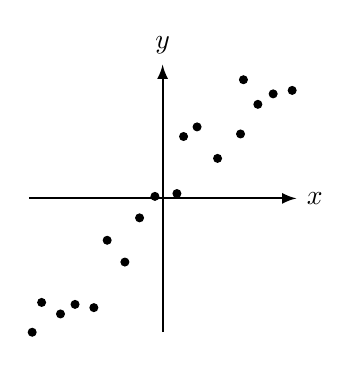
\begin{tikzpicture}
				\draw[->, thick] (-1.7,0)--(1.7,0) node[right]{$x$};
				\draw[->, thick] (0,-1.7)--(0,1.7) node[above]{$y$};
				\foreach \x in {-1.7,-1.5,...,1.7}{
						\pgfmathsetmacro\xcoord{\x+rand/10}
						\pgfmathsetmacro\ycoord{\x+rand/2}
						\pgfmathsetmacro\xcoord{\xcoord < -1.7 ? -1.7 : \xcoord}
						\pgfmathsetmacro\xcoord{\xcoord > 1.7 ? 1.7 : \xcoord}
						\pgfmathsetmacro\ycoord{\ycoord < -1.7 ? -1.7 : \ycoord}
						\pgfmathsetmacro\ycoord{\ycoord > 1.7 ? 1.7 : \ycoord}
						\node[circle,draw,fill=black,scale=0.3] at
						(\xcoord,\ycoord) {};
					}
			\end{tikzpicture}
			\caption{a) Positive correlation.}
		\end{minipage}\hfill
		\begin{minipage}{0.32\textwidth}
			\centering
			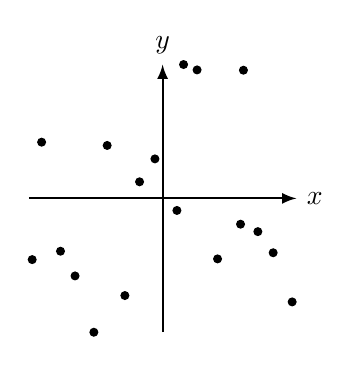
\begin{tikzpicture}
				\draw[->, thick] (-1.7,0)--(1.7,0) node[right]{$x$};
				\draw[->, thick] (0,-1.7)--(0,1.7) node[above]{$y$};
				\foreach \x in {-1.7,-1.5,...,1.7}{
						\pgfmathsetmacro\xcoord{\x+rand/10}
						\pgfmathsetmacro\ycoord{rand*2}
						\pgfmathsetmacro\xcoord{\xcoord < -1.7 ? -1.7 : \xcoord}
						\pgfmathsetmacro\xcoord{\xcoord > 1.7 ? 1.7 : \xcoord}
						\pgfmathsetmacro\ycoord{\ycoord < -1.7 ? -1.7 : \ycoord}
						\pgfmathsetmacro\ycoord{\ycoord > 1.7 ? 1.7 : \ycoord}
						\node[circle,draw,fill=black,scale=0.3] at
						(\xcoord,\ycoord) {};
					}
			\end{tikzpicture}
			\caption{b) Uncorrelated/no correlation.}
		\end{minipage}\hfill
		\begin{minipage}{0.32\textwidth}
			\centering
			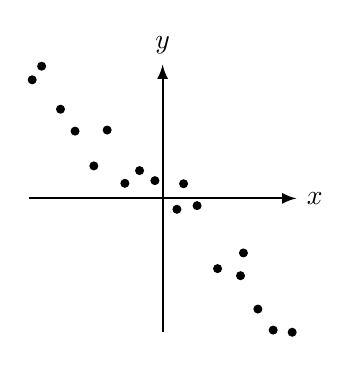
\begin{tikzpicture}
				\draw[->, thick] (-1.7,0)--(1.7,0) node[right]{$x$};
				\draw[->, thick] (0,-1.7)--(0,1.7) node[above]{$y$};
				\foreach \x in {-1.7,-1.5,...,1.7}{
						\pgfmathsetmacro\xcoord{\x+rand/10}
						\pgfmathsetmacro\ycoord{-\x+rand/2}
						\pgfmathsetmacro\xcoord{\xcoord < -1.7 ? -1.7 : \xcoord}
						\pgfmathsetmacro\xcoord{\xcoord > 1.7 ? 1.7 : \xcoord}
						\pgfmathsetmacro\ycoord{\ycoord < -1.7 ? -1.7 : \ycoord}
						\pgfmathsetmacro\ycoord{\ycoord > 1.7 ? 1.7 : \ycoord}
						\node[circle,draw,fill=black,scale=0.3] at
						(\xcoord,\ycoord) {};
					}
			\end{tikzpicture}
			\caption{c) Negative correlation.}
		\end{minipage}\hfill
	\end{figure}
\end{frame}

\begin{frame}{Covariance of Numerical Data (I)}
	\begin{itemize}
		\item \textbf{\color{airforceblue}Covariance} \textbf{is similar to
			      correlation:}\\
		      \begin{align}
			      \text{Cov}(X) =
			      \frac{\sum_{i=1}^{n}(a_i-\mu_{X_a})(b_i-\mu_{X_b})}{\#X} =
			      \frac{\sum_{i=1}^{n}a_ib_i}{\#X}-\mu_{X_a}\mu_{X_b}
		      \end{align}
		\item \textbf{Computing the correlation based on the covariance:}\\
		      \begin{align}
			      \text{Cor}({X}) = \frac{\text{Cov}(X)}{\sigma_{X_a}\sigma_{X_b}}
		      \end{align}
	\end{itemize}
\end{frame}

\begin{frame}{Covariance of Numerical Data (II)}
	\begin{itemize}
		\item \textbf{Positive covariance:}\\
		      If $\text{Cov}(X) > 0$, then $A$ and $B$ tend to be either both
		      larger or both smaller than their expected values.
		\item \textbf{Negative covariance:}\\
		      If $\text{Cov}(X) < 0$, then if $A$ is larger than its expected
		      value, $B$ is likely to be smaller than its expected value and vice
		      versa.
		\item \textbf{Independence:}
		      \begin{itemize}
			      \item $\text{Cov}(X) = 0$.
			      \item \textbf{\color{airforceblue}But the converse is not true:}
			            Some pairs of random variables may have a covariance of $0$ but are
			            not independent. Only under some additional assumptions (e.g., the
			            data follow multivariate normal distributions) does a covariance of
			            $0$ imply independence.
		      \end{itemize}
	\end{itemize}
\end{frame}

\begin{frame}{Covariance: An Example}
	\begin{itemize}
		\item Suppose two stocks being part of $X$ have the following values:\\
		      $(2,5), (3,8), (5,10), (4,11), (6,14).$
		\item If the stocks are affected by the same industry trends, will
		      their prices rise or fall together?
		      \begin{align}
			      \text{Cov}(X) & = \frac{2\cdot5 + 3\cdot 8 + 5 \cdot 10 + 4 \cdot
				      11 + 6 \cdot 14}{5} - 4\cdot 9.6 = 4.
		      \end{align}
		\item Thus, $A$ and $B$ rise together since $\text{Cov}(X) > 0$.
	\end{itemize}
\end{frame}

\section{Data reduction}

\begin{frame}{Data Reduction (I)}
	\begin{itemize}
		\item \textbf{What is data reduction?}\\
		      \begin{itemize}
			      \item Obtain a reduced representation of the data set that is much
			            smaller in volume but yet produces the same (or almost the same)
			            results.
		      \end{itemize}
		\item \textbf{Why data reduction?}\\
		      \begin{itemize}
			      \item A database/data warehouse may store terabytes of data.
			      \item Complex data analysis may take a very long time to run on the
			            complete data set.
		      \end{itemize}
		\item \textbf{Data reduction strategies:}
		      \begin{itemize}
			      \item Dimensionality reduction, i.e. remove unimportant attributes.
			            \begin{itemize}
				            \item Wavelet transforms.
				            \item Principal component analysis.
				            \item Attribute subset selection or attribute creation.
			            \end{itemize}
		      \end{itemize}
	\end{itemize}
\end{frame}

\begin{frame}{Data Reduction (II)}
	\begin{itemize}
		\item \textbf{Data reduction strategies (continued):}
		      \begin{itemize}
			      \item Numerosity reduction:
			            \begin{itemize}
				            \item Regression and log-linear models.
				            \item Histograms, clustering and sampling.
				            \item Data cube aggregation.
			            \end{itemize}
			      \item Data compression.
		      \end{itemize}
	\end{itemize}
\end{frame}

\begin{frame}{Data Reduction (I): Dimensionality Reduction}
	\begin{itemize}
		\item \textbf{Curse of dimensionality:}
		      \begin{itemize}
			      \item When dimensionality increases data becomes increasingly
			            sparse.
			      \item Density and distance between points become less meaningful.
			      \item The possible combinations of subspaces will grow
			            exponentially.
		      \end{itemize}
		\item \textbf{Dimensionality reduction:}
		      \begin{itemize}
			      \item Avoid the curse of dimensionality.
			      \item Help eliminate irrelevant features and reduce noise.
			      \item Reduce time and space required in data mining.
			      \item Allow easier visualization.
		      \end{itemize}
		\item \textbf{Dimensionality-reduction techniques:}
		      \begin{itemize}
			      \item Wavelet transforms.
			      \item Principal component analysis.
			      \item Supervised and nonlinear techniques (e.g. feature selection).
		      \end{itemize}
	\end{itemize}
\end{frame}

\begin{frame}{Wavelet Transform (I)}
	\begin{minipage}[t]{0.55\textwidth}
		\begin{itemize}
			\item \textbf{Decomposes a signal into different frequency
				      subbands.}\\
			      Applicable to $n$-dimensional signals.
			\item Data transformed to preserve relative distance between
			      objects at different levels of resolution.
			\item Allow natural clusters to become more distinguishable.
			\item Used for image compression.
		\end{itemize}
	\end{minipage}\hspace{1cm}
	\begin{minipage}[t]{0.30\textwidth}
		\raisebox{\dimexpr-\height+\ht\strutbox\relax}{\includegraphics[width=5cm]{img/wavelettransform.png}}
	\end{minipage}
\end{frame}

\begin{frame}{Wavelet Transform (II)}
	\begin{itemize}
		\item \textbf{Discrete wavelet transform:}\\
		      Transforms a vector $X$ into a different vector $X'$ of wavelet
		      coefficients with the same length.
		\item \textbf{Compressed approximation:}\\
		      Store only a small fraction of the strongest of the wavelet
		      coefficients.
		\item \textbf{Similar to discrete fourier transform, but better lossy
			      compression, localized in space.}
		\item \textbf{Method:}
		      \begin{itemize}
			      \item The length of the vector must be an integer power of $2$
			            (padding with $0$'s if necessary).
			      \item Each transform has two functions: smoothing and difference.
			      \item Applied to pairs of data, resulting in two sets of data with
			            half the length.
			      \item The two functions are applied recursively until reaching the
			            desired length.
		      \end{itemize}
	\end{itemize}
\end{frame}

\begin{frame}{Example: Wavelet Transform (I)}
	\begin{itemize}
		\item \textbf{Initial vector:}
		      \begin{itemize}
			      \item $X = (2,2,0,2,3,5,4,4)$
		      \end{itemize}
		\item \textbf{First step:}
		      \begin{itemize}
			      \item $(2,2) \rightarrow \text{Average: } 2, \text{Weighted
					            difference: } 0$
			      \item $(0,2) \rightarrow \text{Average: } 1, \text{Weighted
					            difference: } -1$
			      \item $(3,5) \rightarrow \text{Average: } 4, \text{Weighted
					            difference: } -1$
			      \item $(4,4) \rightarrow \text{Average: } 4, \text{Weighted
					            difference: } 0$
			      \item $A_1=(2,1,4,4), D_1=(0,-1,-1,0)$
		      \end{itemize}
		\item \textbf{Second step:}
		      \begin{itemize}
			      \item $(2,1) \rightarrow \text{Average: } 1.5, \text{Weighted
					            difference: } 0.5$
			      \item $(4,4) \rightarrow \text{Average: } 4, \text{Weighted
					            difference: } 0$
			      \item $A_2=(1.5,4), D_2=(0.5,0)$
		      \end{itemize}
	\end{itemize}
\end{frame}

\begin{frame}{Example: Wavelet Transform (II)}
	\begin{itemize}
		\item \textbf{Third step:}
		      \begin{itemize}
			      \item $(1.5,4) \rightarrow \text{Average: } 2.75, \text{Weighted
					            difference: } -1.25$
			      \item $A_3=(2.75), D_3=(-1.25)$
		      \end{itemize}
		\item \textbf{Resulting vector:}
		      \begin{itemize}
			      \item $X' = (2.75,-1.25,0.5,0,0,-1,-1,0)$
		      \end{itemize}
		\item \textbf{Possible compression:}\\
		      \begin{itemize}
			      \item Small detail coefficients ($D_{1,2,3}$) can be replaced by
			            $0$'s,
			            while retaining significant coefficients.
		      \end{itemize}
	\end{itemize}
	\vspace{0.2cm}
	\centering
	\begin{tabular}{|c|c|c|}
		\hline
		\text{Resolution} & \text{Averages}     & \text{Detail coefficients}
		\\\hline
		$8$               & $(2,2,0,2,3,5,4,4)$ & -
		\\\hline
		$4$               & $(2,1,4,4)$         & $(0,-1,-1,0)$
		\\\hline
		$2$               & $(1.5,4)$           & $(0.5,0)$
		\\\hline
		$1$               & $(2.75)$            & $(-1.25)$
		\\\hline
	\end{tabular}
\end{frame}

\begin{frame}{Why Wavelet Transform?}
	\begin{itemize}
		\item \textbf{Hat-shaped filters:}
		      \begin{itemize}
			      \item Emphasize region where points cluster.
			      \item Suppress weaker information in their boundaries.
		      \end{itemize}
		\item \textbf{Effective removal of outliers:}
		      \begin{itemize}
			      \item Insensitive to noise, insensitive to input order.
		      \end{itemize}
		\item \textbf{Multi-resolution:}
		      \begin{itemize}
			      \item Detect arbitrary shaped clusters at different scales.
		      \end{itemize}
		\item \textbf{Efficient:} Complexity $\mathcal{O}(N)$.
	\end{itemize}
\end{frame}

\begin{frame}{Principal Component Analysis (PCA)}
	\begin{itemize}
		\item \textbf{Main idea:}
		      \begin{itemize}
			      \item Given a data set with $n$ dimensions.
			      \item Find $k \leq n$ orthogonal vectors that capture the largest
			            amount of data.
			      \item Works only for numeric data.
		      \end{itemize}
		\item \textbf{Example data set:}
		      \begin{itemize}
			      \item Used on the next few slides to explain the steps of a PCA:
		      \end{itemize}
		      \vspace{3mm}
		      \centering
		      \begin{tabular}{|c|c|c|}
			      \hline
			      $d_1$ & $d_2$ & $d_3$
			      \\\hline
			      $23$  & $6$   & $1$
			      \\\hline
			      $9$   & $9$   & $5$
			      \\\hline
			      $17$  & $5$   & $1$
			      \\\hline
			      $3$   & $6$   & $1$
			      \\\hline
		      \end{tabular}
	\end{itemize}
\end{frame}

\begin{frame}{Principal Component Analysis - 1. Step: Standardization (I)}
	\begin{itemize}
		\item \textbf{Procedure:}
		      \begin{itemize}
			      \item Each value $x$ within a dimension $d_n$ is standardized with
			            the help of the mean ($\mu_{d_n}$) and standard deviation
			            ($\sigma_{d_n}$) of $d_n$:
			            \begin{align*}
				            x' = \frac{x - \mu_{d_n}}{\sigma_{d_n}}
			            \end{align*}
		      \end{itemize}
		\item \textbf{Reason:}
		      \begin{itemize}
			      \item Each dimension should be considered equally in the analysis.
			      \item Dimensions with a wider range of	values would dominate
			            without this step.
		      \end{itemize}
	\end{itemize}
\end{frame}

\begin{frame}{Principal Component Analysis - 1. Step: Standardization (II)}
	\begin{itemize}
		\item \textbf{Example:}
		      \begin{itemize}
			      \item Mean and standard deviation per dimension: \\
			            \vspace{3mm}
			            \begin{center}
				            \centering
				            \begin{tabular}{|l|c|c|c|}
					            \hline
					                     & $d_1$       & $d_2$      & $d_3$ \\
					            \hline
					            $\mu$    & $13.000000$ & $6.500000$ & $2.0$ \\
					            \hline
					            $\sigma$ & $8.793937$  & $1.732051$ & $2.0$ \\
					            \hline
				            \end{tabular}
			            \end{center}
			            \vspace{3mm}
			      \item Standardized data set: \\
			            \vspace{3mm}
			            \begin{center}
				            \centering
				            \begin{tabular}{|c|c|c|}
					            \hline
					            $d_1$       & $d_2$       & $d_3$
					            \\\hline
					            $+1.137147$ & $-0.288675$ & $-0.5$
					            \\\hline
					            $-0.454859$ & $+1.443376$ & $+1.5$
					            \\\hline
					            $+0.454859$ & $-0.866025$ & $-0.5$
					            \\\hline
					            $-1.137147$ & $-0.288675$ & $-0.5$
					            \\\hline
				            \end{tabular}
			            \end{center}
		      \end{itemize}
	\end{itemize}
\end{frame}

\begin{frame}{Principal Component Analysis - 2. Step: Covariance Matrix (I)}
	\begin{itemize}
		\item \textbf{Procedure:}
		      \begin{itemize}
			      \item A n x n covariance matrix is generated that contains the
			            covariance between each possible attribute pairing. When the
			            dimensions are compared with themselves, the variance always
			            replaces the covariance:
			            \begin{align*}
				            \begin{bmatrix}
					            \text{Var}(d_1)      & ... & \text{Cov}(d_1, d_n) \\
					            ...                  & ... & ...                  \\
					            \text{Cov}(d_n, d_1) & ... & \text{Var}(d_n)      \\
				            \end{bmatrix}
			            \end{align*}
		      \end{itemize}
		\item \textbf{Reason:}
		      \begin{itemize}
			      \item Dimensions that are highly correlated contain redundant
			            information.
			      \item This step helps to identify these correlations.
		      \end{itemize}
	\end{itemize}
\end{frame}

\begin{frame}{Principal Component Analysis - 2. Step: Covariance Matrix (II)}
	\begin{itemize}
		\item \textbf{Example:}
		      \begin{itemize}
			      \item The 3 x 3 covariance matrix of our example: \\
			            \vspace{3mm}
			            \begin{center}
				            \centering
				            \begin{tabular}{|l|c|c|c|}
					            \hline
					                  & $d_1$       & $d_2$       & $d_3$
					            \\\hline
					            $d_1$ & $+1.000000$ & $-0.350150$ & $-0.303239$
					            \\\hline
					            $d_2$ & $-0.350150$ & $+1.000000$ & $+0.962250$
					            \\\hline
					            $d_3$ & $-0.303239$ & $+0.962250$ & $+1.000000$
					            \\\hline
				            \end{tabular}
			            \end{center}
		      \end{itemize}
	\end{itemize}
\end{frame}

\begin{frame}{Principal Component Analysis - 3. Step: Eigenvalues (I)}
	\begin{itemize}
		\item \textbf{Procedure:}
		      \begin{itemize}
			      \item The eigenvectors and eigenvalues of the covariance matrix
			            ($C$) are computed by solving the following equation:
			            \begin{align*}
				            C \nu = \lambda \nu
			            \end{align*}
			      \item If an n digit vector $\nu$ satisfies this equation for a
			            $\lambda \in \mathbb{R}$, then $\nu$ is called an eigenvector with
			            associated eigenvalue $\lambda$
		      \end{itemize}
		\item \textbf{Reason:}
		      \begin{itemize}
			      \item The determined eigenvectors are called \textbf{prinicipal
				            components} of the dataset. The eigenvalues indicate which of these
			            prinicipal components has which importance for the significance of
			            the dataset.
			      \item By sorting the eigenvectors in descending order according to
			            their eigenvalues, the prinicipal components that contain the most
			            information can be identified.
		      \end{itemize}
	\end{itemize}
\end{frame}

\begin{frame}{Principal Component Analysis - 3. Step: Eigenvalues (II)}
	\begin{itemize}
		\item \textbf{Example:}
		      \begin{itemize}
			      \item Eigenvalues and eigenvectors in our example: \\
			            \begin{align*}
				            \lambda_1 = +2.14823654,
				            \nu_1 = \begin{bmatrix} +0.37342507 \\ -0.92684562 \\ -0.03887043 \end{bmatrix}
				            \\
				            \lambda_2 = +0.81530433,
				            \nu_2 = \begin{bmatrix} -0.66009198 \\ -0.23604255 \\ -0.71313568 \end{bmatrix}
				            \\
				            \lambda_3 = +0.03645914,
				            \nu_3 = \begin{bmatrix} -0.6517916 \\ -0.2919608 \\ +0.69994757 \end{bmatrix}
			            \end{align*}
			      \item Sorting these three eigenvectors by their significance, we
			            arrive at the order $\nu_1$, $\nu_2$, $\nu_3$
		      \end{itemize}
	\end{itemize}
\end{frame}

\begin{frame}{Principal Component Analysis - 4. Step: Feature matrix (I)}
	\begin{itemize}
		\item \textbf{Procedure:}
		      \begin{itemize}
			      \item The top N eigenvectors are selected to create a feature
			            matrix from them.
			      \item There is no fixed rule exactly how many eigenvectors should
			            be selected.
			      \item The dimensionality reduction is larger the
			            fewer eigenvectors are chosen.
			      \item The information loss increases with each eigenvector that is
			            discarded.
		      \end{itemize}
		\item \textbf{Reason:}
		      \begin{itemize}
			      \item It must be considered carefully how much information can be
			            given up in favor of dimensionality reduction.
		      \end{itemize}
	\end{itemize}
\end{frame}

\begin{frame}{Principal Component Analysis - 4. Step: Feature matrix (II)}
	\begin{itemize}
		\item \textbf{Example:}
		      \begin{itemize}
			      \item In our example $\nu_1$ carries approx. $72\%$ of the
			            information: \\
			            \begin{align*}
				            \frac{2.14823654}{2,14823654+0,81530433+0,03645914} = 0.71607885
			            \end{align*}
			      \item It might be interesting to keep only the eigenvector $\nu_1$
			            and discard the other two eigenvectors. Our feature matrix
			            therefore looks as follows:
			            \begin{align*}
				            \begin{bmatrix} +0.37342507 \\ -0.92684562 \\ -0.03887043 \end{bmatrix}
			            \end{align*}
		      \end{itemize}
	\end{itemize}
\end{frame}

\begin{frame}{Principal Component Analysis - 5. Step: Transformation (I)}
	\begin{itemize}
		\item \textbf{Procedure:}
		      \begin{itemize}
			      \item The original data set ($D$) gets multiplied with the feature
			            matrix ($F$), to create a new data set ($N$) with lower
			            dimensionality:
			            \begin{align*}
				            N = D \cdot F
			            \end{align*}
		      \end{itemize}
		\item \textbf{Reason:}
		      \begin{itemize}
			      \item This step applies the dimensionality reduction to each tuple.
			      \item The PCA is completed with this step.
		      \end{itemize}
	\end{itemize}
\end{frame}

\begin{frame}{Principal Component Analysis - 5. Step: Transformation (II)}
	\begin{itemize}
		\item \textbf{Example:}
		      \begin{itemize}
			      \item Our dataset after the transformation and with the PCA
			            completed looks like this: \\
			            \begin{align*}
				            \begin{bmatrix} +0.711632 \\ -1.565948 \\ +0.991963 \\ -0.137647
				            \end{bmatrix}
			            \end{align*}
			      \item It is to be expected that this dataset still contains about
			            $72\%$ of its original information, which can be
			            further used for data mining, while having to deal with
			            a lot less dimensions.
		      \end{itemize}
	\end{itemize}
\end{frame}

\begin{frame}{Attribute-subset Selection}
	\begin{itemize}
		\item \textbf{Another way to reduce dimensionality of data.}
		      \item\textbf{\color{airforceblue}Redundant attributes:}
		      \begin{itemize}
			      \item Duplicate much or all of the information contained in other
			            attributes.
			            \begin{itemize}
				            \item E.g. purchase price of a product and the amount of sales
				                  tax paid.
			            \end{itemize}
		      \end{itemize}
		\item \textbf{\color{airforceblue}Irrelevant attributes:}
		      \begin{itemize}
			      \item contain no information that is useful for the data-mining
			            task at hand.
			            \begin{itemize}
				            \item E.g. students' ID is often irrelevant to the task of
				                  predicting students' GPA.
			            \end{itemize}
		      \end{itemize}
	\end{itemize}
\end{frame}

\begin{frame}{Heuristic Search in Attribute Selection}
	\begin{itemize}
		\item \textbf{There are $2^d$ possible attribute combinations of $d$
			      attributes.}
		      \item\textbf{\color{airforceblue}Typical heuristic attribute-selection
			      methods:}
		      \begin{itemize}
			      \item Best single attribute under the attribute-independence
			            assumption: \\ choose by significance tests (e.g. t-test, see
			            Chapter 6).
			      \item Best step-wise feature selection:
			            \begin{itemize}
				            \item The best single attribute is picked first.
				            \item Then next best attribute condition to the first \ldots
			            \end{itemize}
		      \end{itemize}
		\item \textbf{\color{airforceblue}Step-wise attribute elimination:}
		      \begin{itemize}
			      \item Repeatedly eliminate the worst attribute.
		      \end{itemize}
		\item Best combined attribute selection and elimination.
		\item Optimal branch and bound:
		      \begin{itemize}
			      \item Use attribute elimination and backtracking.
		      \end{itemize}
	\end{itemize}
\end{frame}

\begin{frame}{Attribute Creation (Feature Generation)}
	\begin{itemize}
		\item \textbf{Create new attributes (features) that can capture the
			      important information in a data set more effectively than the original
			      ones.}
		\item \textbf{Three general methodologies:}
		      \begin{itemize}
			      \item Attribute extraction.
			            \begin{itemize}
				            \item Domain-specific.
			            \end{itemize}
			      \item Mapping data to new space (see: data reduction).
			            \begin{itemize}
				            \item E.g. Fourier transformation, wavelet transformation,
				                  manifold approaches (not covered).
			            \end{itemize}
			      \item Attribute construction:
			            \begin{itemize}
				            \item Combining features (see: discriminative frequent patterns
				                  in Chapter 5).
				            \item Data discretization.
			            \end{itemize}
		      \end{itemize}
	\end{itemize}
\end{frame}

\begin{frame}{Data Reduction (II): Numerosity Reduction}
	\begin{itemize}
		\item \textbf{Reduce data volume by choosing alternative,
			      {\color{airforceblue}smaller} forms of data representation.}
		\item \textbf{{\color{airforceblue}Parametric} methods (e.g.,
			      regression):}
		      \begin{itemize}
			      \item Assume the data fits some
			            \textbf{{\color{airforceblue}model}} (e.g. a function).
			      \item Estimate model parameters.
			      \item Store only the parameters.
			      \item Discard the data (except possible outliers):
			            \begin{itemize}
				            \item Ex. log-linear models obtain value at a point in
				                  $m$-dimensional space as the product of appropriate marginal
				                  subspaces.
			            \end{itemize}
		      \end{itemize}
		\item \textbf{{\color{airforceblue}Non-parametric} methods:}
		      \begin{itemize}
			      \item Do not assume models.
			      \item Major families: histograms, clustering, sampling, \ldots
		      \end{itemize}
	\end{itemize}
\end{frame}

\begin{frame}{Histogram Analysis}
	\begin{itemize}
		\item \textbf{Divide data into buckets and store average (sum) of each
			      bucket.}
		\item \textbf{Partitioning rules:}
		      \begin{itemize}
			      \item Equal-width: equal bucket range.
			      \item Equal-frequency (or equal-depth).
		      \end{itemize}
	\end{itemize}
	\centering
	\includegraphics[width=9.5cm]{img/histogram.png}
\end{frame}

\begin{frame}{Clustering}
	\begin{itemize}
		\item \textbf{Partition data set into clusters based on similarity and
			      store cluster representation (e.g., centroid and diameter) only.}
		      \begin{itemize}
			      \item Can be very effective if data points are close to each other
			            under a certain norm and choice of space.
			      \item Can have hierarchical clustering and be stored in
			            multidimensional index-tree structures.
			      \item There are many choices of clustering algorithms.
			      \item Cluster analysis will be studied in depth in Chapter 7.
		      \end{itemize}
	\end{itemize}
\end{frame}

\begin{frame}{Sampling}
	\begin{itemize}
		\item \textbf{Obtain a small sample $x$ to represent the whole data set
			      $X$.}
		\item \textbf{Allow a mining algorithm to run in complexity \\ that is
			      potentially sub-linear to the size of the data.}
		\item \textbf{Key principle: Choose a
				      {\color{airforceblue}representative} subset of the data.}
		      \begin{itemize}
			      \item Simple random sampling may have very poor performance in the
			            presence of skew.
			      \item Develop adaptive sampling methods, e.g. stratified sampling.
		      \end{itemize}
		\item \textbf{Note: Sampling may not reduce database I/Os.}
		      \begin{itemize}
			      \item One page at a time.
		      \end{itemize}
	\end{itemize}
\end{frame}

\begin{frame}{Types of Sampling}
	\begin{itemize}
		\item \textbf{Simple random sampling.}
		      \begin{itemize}
			      \item There is an equal probability of selecting any particular
			            item.
		      \end{itemize}
		\item \textbf{Sampling without replacement.}
		      \begin{itemize}
			      \item Once an object is selected, it is removed from the population.
		      \end{itemize}
		\item \textbf{Sampling with replacement.}
		      \begin{itemize}
			      \item A selected object is not removed from the population.
		      \end{itemize}
		\item \textbf{Stratified sampling:}
		      \begin{itemize}
			      \item Partition the data set and draw samples from each partition:
			            Proportionally, i.e. approximately the same percentage of the data.
			      \item Used in conjunction with skewed data.
		      \end{itemize}
	\end{itemize}
\end{frame}

\begin{frame}{Data-cube Aggregation}
	\begin{itemize}
		\item \textbf{The lowest level of a data cube (base cuboid).}
		      \begin{itemize}
			      \item The aggregated data for an \textbf{individual entity of
				            interest}.
			      \item E.g. a customer in a phone-calling data warehouse.
			      \item Number of calls per hour, day, or week.
		      \end{itemize}
		\item \textbf{Multiple levels of aggregation in data cubes.}
		      \begin{itemize}
			      \item Further reduce the size of data to deal with.
		      \end{itemize}
		\item \textbf{Reference appropriate levels.}
		      \begin{itemize}
			      \item Use the smallest representation that is enough to solve
			            the task.
		      \end{itemize}
		\item \textbf{Queries regarding aggregated information should be
			      answered using the data cube, if possible.}
	\end{itemize}
\end{frame}

\begin{frame}{Data Reduction (III): Data Compression}
	\begin{itemize}
		\item \textbf{String compression.}
		      \begin{itemize}
			      \item There are extensive theories and well-tuned algorithms.
			      \item Typically lossless, but only limited manipulation is possible
			            without expansion.
		      \end{itemize}
		\item \textbf{Audio/video compression.}
		      \begin{itemize}
			      \item Typically lossy compression, with progressive refinement.
			      \item Sometimes small fragments of signal can be reconstructed
			            without reconstructing the whole.
		      \end{itemize}
		\item \textbf{Time sequence is not audio.}
		      \begin{itemize}
			      \item Typically short and varies slowly with time.
		      \end{itemize}
		\item \textbf{Dimensionality and numerosity reduction may also be
			      considered as forms of data compression.}
	\end{itemize}
\end{frame}

\section{Data Transformation and Data Discretization}

\begin{frame}{Data Transformations}
	\begin{itemize}
		\item Functions applied to a finite set of samples.
		\item \textbf{Methods:}
		      \begin{itemize}
			      \item Smoothing: Remove noise from data.
			      \item Attribute/feature construction: New attributes constructed
			            from the given ones.
			      \item Aggregation: Summarization, data-cube construction.
			      \item Normalization: Scaled to fall within a smaller, specified
			            range.
			            \begin{itemize}
				            \item Min-max normalization
				            \item Z-score normalization.
				            \item Normalization by decimal scaling.
			            \end{itemize}
			      \item Discretization: concept-hierarchy climbing.
		      \end{itemize}
	\end{itemize}
\end{frame}

\begin{frame}{Normalization}
	\begin{itemize}
		\item \textbf{Min-max normalization (to some interval
			      $[\text{min},\text{max}]$):}
		      \begin{align*}
			      a_{\text{new}} = \frac{a - \text{min}_A}{\text{max}_A-\min_{A}}
			      (\max - \min) + \min.
		      \end{align*}
		      Example: let income range from $\$12,000$ to $\$98,000$ normalized to
		      $[0,1]$.\\
			      Then $\$73,600$ is mapped to $\frac{73,600-12,000}{98,000-12,000} (1-0)
		      + 0 = 0.716$.
		\item \textbf{Z-score normalization:}
		      \begin{align*}
			      a_{\text{new}} := z(a) = \frac{a-\mu_{A}}{\sigma_A}, \; \text{with
				      $\mu$ being the mean and $\sigma$ the standard deviation.}
		      \end{align*}
		      Example: let $\mu = 54,000$ and $\sigma = 16,000$. Then
		      $\frac{73,000-54,000}{16,000} = 1.188$.
		\item \textbf{Normalization by decimal scaling:}
		      \begin{align*}
			      a_{\text{new}} = \frac{a}{10^k}, \; \text{where $k$ is the smallest
				      integer such that} \; \max(\vert a_{\text{new}} \vert) < 1.
		      \end{align*}
	\end{itemize}
\end{frame}

\begin{frame}{Discretization}
	\begin{itemize}
		\item \textbf{Three types of attributes:}
		      \begin{itemize}
			      \item Nominal -- values from an unordered set, e.g. color,
			            profession.
			      \item Ordinal -- values from an ordered set, e.g. military or
			            academic rank.
			      \item Numerical -- numbers, e.g. integer or real numbers.
		      \end{itemize}
		\item \textbf{Divide the value range of a continuous attribute into
			      intervals:}
		      \begin{itemize}
			      \item \textbf{Interval labels} can then be used to replace actual
			            data values.
			      \item Reduce data size by discretization.
			      \item Supervised vs. unsupervised.
			      \item Split (top-down) vs. merge (bottom-up).
			      \item Discretization can be performed recursively on an attribute.
			      \item Prepare for further analysis, e.g. classification.
		      \end{itemize}
	\end{itemize}
\end{frame}

\begin{frame}{Data-Discretization Methods}
	\begin{itemize}
		\item \textbf{Typical methods:}
		      \begin{itemize}
			      \item All the methods can be applied recursively.
			      \item \textbf{Binning:}
			            \begin{itemize}
				            \item Unsupervised, top-down split.
			            \end{itemize}
			      \item \textbf{Histogram analysis:}
			            \begin{itemize}
				            \item Unsupervised, top-down split.
			            \end{itemize}
			      \item \textbf{Clustering analysis:}
			            \begin{itemize}
				            \item Unsupervised, top-down split or bottom-up merge.
			            \end{itemize}
			      \item \textbf{Decision-tree analysis:}
			            \begin{itemize}
				            \item Supervised, top-down split.
			            \end{itemize}
			      \item \textbf{Correlation (e.g. $\chi^2$) analysis:}
			            \begin{itemize}
				            \item Unsupervised, bottom-up merge.
			            \end{itemize}
		      \end{itemize}
	\end{itemize}
\end{frame}

\begin{frame}{Simple Discretization: Binning}
	\begin{itemize}
		\item \textbf{Equal-width (distance) partitioning:}
		      \begin{itemize}
			      \item Divides the range into $N$ intervals of equal size: uniform
			            grid.
			      \item If $A$ and $B$ are the lowest and highest values of the
			            attribute, the width of intervals will be: $W = \frac{(B - A)}{N}$.
			      \item The most straightforward, but outliers may dominate
			            presentation.
			      \item Skewed data is not handled well.
		      \end{itemize}
		\item \textbf{Equal-depth (frequency) partitioning:}
		      \begin{itemize}
			      \item Divides the range into $N$ intervals, each containing
			            approximately the same number of samples.
			      \item Good data scaling.
			      \item Managing categorical attributes can be tricky.
		      \end{itemize}
	\end{itemize}
\end{frame}

\begin{frame}{Binning Methods for Data Smoothing}
	\begin{itemize}
		\item \textbf{Sorted data for price (in dollars):} \\
		      $4, 8, 9, 15, 21, 21, 24, 25, 26, 28, 29, 34$.
		\item \textbf{Partition into equal-frequency (equal-depth) bins:}\\
		      Bin $1$: $4, 8, 9, 15$,\\
		      Bin $2$: $21, 21, 24, 25$,\\
		      Bin $3$: $26, 28, 29, 34$.
		\item \textbf{Smoothing by bin means:}\\
		      Bin $1$: $9, 9, 9, 9$,\\
		      Bin $2$: $23, 23, 23, 23$,\\
		      Bin $3$: $29, 29, 29, 29$.\\
		\item \textbf{Smoothing by bin boundaries:}\\
		      Bin $1$: $4, 4, 4, 15$,\\
		      Bin $2$: $21, 21, 25, 25$,\\
		      Bin $3$: $26, 26, 26, 34$.\\
	\end{itemize}
\end{frame}

\begin{frame}{Binning vs. Clustering}
	\begin{figure}[H]
		\centering
		\begin{minipage}{0.32\textwidth}
			\includegraphics[width=5cm]{img/binningvsclustering2.png}
			\caption{a) Equal interval width (binning).}
		\end{minipage}
		\begin{minipage}{0.32\textwidth}
			\centering
			\includegraphics[width=5cm]{img/binningvsclustering3.png}
			\caption{b) Equal frequency (binning).}
		\end{minipage}
		\begin{minipage}{0.32\textwidth}
			\centering
			\includegraphics[width=5cm]{img/binningvsclustering4.png}
			\caption{c) K-means clustering.}
		\end{minipage}\hfill
	\end{figure}
\end{frame}

\begin{frame}{Classification \& Correlation Analysis}
	\begin{itemize}
		\item \textbf{Classification:}
		      \begin{itemize}
			      \item E.g. decision-tree analysis.
			      \item Supervised: Class labels given for training set e.g.
			            cancerous vs. benign.
			      \item Using \textbf{entropy} to determine split point
			            (discretization point).
			      \item Top-down, recursive split.
			      \item Details will be covered in Chapter 6.
		      \end{itemize}
		\item \textbf{Correlation analysis:}
		      \begin{itemize}
			      \item E.g. $\chi^2$-merge: $\chi^2$-based discretization.
			      \item Supervised: use class information.
			      \item Bottom-up merge: find the best neighboring intervals (those
			            having similar distributions of classes, i.e., low $\chi^2$ values)
			            to merge.
			      \item Merge performed recursively, until a predefined stopping
			            condition.
		      \end{itemize}
	\end{itemize}
\end{frame}

\begin{frame}{Concept-hierarchy Generation}
	\begin{itemize}
		\item \textbf{Concept hierarchy:}
		      \begin{itemize}
			      \item Organizes concepts (i.e. attribute values) hierarchically.
			      \item Usually associated with each dimension in a data warehouse.
			      \item Facilitates \textbf{drilling and rolling} in data warehouses
			            to view data at multiple granularity.
		      \end{itemize}
		\item \textbf{Concept-hierarchy formation:}
		      \begin{itemize}
			      \item Recursively reduce the data by collecting and replacing
			            \textbf{low-level concepts} (such as numerical values for age) by
			            \textbf{higher-level concepts} (such as youth, adult, or senior).
			      \item Can be explicitly specified by domain experts and/or
			            data-warehouse designers.
			      \item Can be automatically formed for both numerical and nominal
			            data.
			      \item For numerical data, use discretization methods shown.
		      \end{itemize}
	\end{itemize}
\end{frame}

\begin{frame}{Concept-hierarchy Generation for Nominal Data}
	\begin{itemize}
		\item \textbf{Specification of a partial/total ordering of attributes
			      explicitly at the schema level by users or experts.}
		      \begin{itemize}
			      \item $\#(\text{streets}) \prec \#(\text{city}) \prec
				            \#(\text{state}) \prec \#(\text{country})$.
		      \end{itemize}
		\item \textbf{Specification of a hierarchy for a set of values by
			      explicit data grouping.}
		      \begin{itemize}
			      \item $\#(\{"Urbana", "Champaign", "Chicago"\}) \prec
				            \#(\text{Illinois})$.
		      \end{itemize}
		\item \textbf{Specification of only a partial set of attributes.}
		      \begin{itemize}
			      \item Only $\#(\text{street}) \prec \#(\text{city})$, not others.
		      \end{itemize}
		\item \textbf{Automatic generation of hierarchies (or attribute levels)
			      by the analysis of the number of distinct values.}
		      \begin{itemize}
			      \item E.g. for a set of attributes: $\{\text{street}, \text{city},
				            \text{state}, \text{country}\}$.
			      \item See on the next slides.
		      \end{itemize}
	\end{itemize}
\end{frame}

\begin{frame}{Automatic Concept-hierarchy Generation}
	\begin{itemize}
		\item \textbf{Some hierarchies can be automatically generated based on
			      the analysis of the number of distinct values per attribute.}
		      \begin{itemize}
			      \item The attribute with the most distinct values is placed at the
			            lowest level of the hierarchy.
			      \item Exceptions, e.g. weekday, month, quarter, year.
		      \end{itemize}
		\item Example:
		      \begin{align*}
			      \#(\text{streets})           & = 674.339 > \#(\text{city}) =
			      3567,                                                         \\
			      \#(\text{city})              & =  3567 > \#(\text{province or
			      state}) =  356,                                               \\
			      \#(\text{province or state}) & =  356 > \#(\text{country}) =
			      15.
		      \end{align*}
	\end{itemize}
\end{frame}

\section{Summary}

\begin{frame}{Summary}
	\begin{itemize}
		\item \textbf{Data quality:} Accuracy, completeness, consistency, 
		timeliness, believability, interpretability.
		\item \textbf{Data cleaning:} E.g. missing/noisy values, outliers.
		\item \textbf{Data integration from multiple sources:}
		\begin{itemize}
			\item Entity identification problem.
			\item Remove redundancies.
			\item Detect inconsistencies.
		\end{itemize}
		\item \textbf{Data reduction:}
		\begin{itemize}
			\item Dimensionality reduction.
			\item Numerosity reduction.
			\item Data compression.
		\end{itemize}
		\item \textbf{Data transformation and data discretization:}
		\begin{itemize}
			\item Normalization.
			\item Concept-hierarchy generation.
		\end{itemize}
	\end{itemize}
\end{frame}
\begin{frame}[c]
	\begin{center}
		{\bf Any questions about this chapter?}\\[0.5cm]
		Ask them now or ask them later in our forum: \\\bigskip
		StudOn Forum \\
		\faLink\ \url{https://www.studon.fau.de/frm5045379.html} \smallskip

	\end{center}
\end{frame}


\end{document}
